We begin with a short set of assumptions: that the DM particle, $\chi$, is a weakly interacting Dirac fermion, that it is a singlet under the SM, and that it is the lightest stable new particle. We also require minimal flavour violation (MVF) to hold wherever relevant. (\comm{Not sure if this is relevant anymore, if we've ditched the scalar model. - Mia}) Each model is built around a scenario whereby $\chi$ and SM quarks are coupled via a mediator. Coupling to SM leptons \cite{} or gluons \cite{} is beyond the scope of this paper, but these cases have been studied elsewhere. Resolving the contact interaction of an EFT at tree-level leads to two possibilities: the mediating particle is exchanged in the $s$-channel, in which case it is also a SM singlet, or it is exchanged in the $t$-channel, in which case it is necessarily charged and coloured. With these assumptions in mind, two $s$-channel models and one $t$-channel model were chosen for analysis. 

The $s$-channel models are characterised by vector (sV) or axial-vector (sA) couplings to both the dark and SM sectors. In the notation of Ref.~\cite{DMCons2}, these correspond to the D5 and D8 operators respectively in the EFT regime. These models are described by the following interaction Lagrangians:
\begin{equation}
\label{L_int_sV}
\mathcal{L}_{sV} = - \xi_{\mu}\left[ \sum\limits_{q} g_{q}\bar{q}\gamma^{\mu}q - g_{\chi}\bar{\chi}\gamma^{\mu}\chi\right],
\end{equation}
\begin{equation}
\label{L_int_sA}
\mathcal{L}_{sA} =  \xi_{\mu}\left[\sum\limits_{q} g_{q}\bar{q}\gamma^{\mu}\gamma_{5}q - g_{\chi}\bar{\chi}\gamma^{\mu}\gamma_{5}\chi\right],
\end{equation}
%\begin{equation}
%\label{L_int_sS}
%\mathcal{L}_{sS} = \sum\limits_{i=1}^{6} g_{q_i}\bar{q_i}q_i\eta + g_{\chi}\bar{\chi}\chi\eta,
%\end{equation}
\st{where the sum is over all quarks, $\xi$ is the (axial-)vector mediator and $\chi$ is the dark matter particle - a weakly interacting SM singlet Dirac fermion with mass $m_{\chi}$.}
%\question{The scalar model should really have a Yukawa coupling (ie $g_q \rightarrow g_q m_q / v$) if we want to be consistent with D1 and the ATLAS/CMS run2 simplified models. Is it too late to implement this? - Tom.} \comm{I agree, and this should be easy enough to implement I think. - Amelia} 
%\st{For simplicity, it is assumed that both $\xi$ and $\eta$ are SM singlet particles and couple only to pair-antipair combinations of $\chi$ and the SM quarks, with coupling strengths $g_{\chi}$ and $g_q$ respectively.} 
For the couplings $g_q$ and $g_{\chi}$ to remain within the perturbative regime, they are required to satisy $g_{q},g_{\chi} \leq 4\pi$, though stronger perturbativity requirements do exist \cite{ValidEFT}.
%\bigskip

%\st{Finally, for convenience, the mediator is assumed to couple to }$\cancel{\chi}$\st{ with the same strength as to each of the six quarks, that is, }$\cancel{g_{q} = g_{\chi} \equiv f}$. \comm{Removed, since we want to include cases where this isn't true! - Amelia} 
%Note that the vector and axial-vector models have already been studied extensively \cite{Buchmueller:2014yoa, Chatrchyan:2013qha, Aad:2012hf, Harris:2014hga} and so serve as a good basis for the comparison of constraints. \comm{I need to add some citations for the scalar model here - Tom}

The last model considered in this paper, a $t$-channel scalar mediator model (which we refer to by the descriptor tS), juxtaposes nicely with the $s$-channel models. In the heavy-mediator limit, it is converted into a combination of the D5 and D8 EFT operators via Fierz transformation. In addition, the tS model is motivated by analogy with a common aspect of Supersymmetric models: neutralino DM interacting with the SM sector via $t$-channel exchange of a squark\footnote{Note that in the Supersymmetric scenario the DM particle is a Majorana fermion. Simplified models in which the DM particle is a Majorana fermion are not covered here (the exception being in the validation of the mono-$Z$ channel, see sec.\ref{monoZ_validation}) as they are kinematically identical to the corresponding Dirac cases, and only require multiplication of the cross-section by a simple factor in order to calculate limits. The exception to this rule is the $s$-channel vector mediator model, which vanishes if $\chi$ is a Majorana fermion \cite{METSig}.} \cite{SUSYDM}.
%\bigskip

In this model, the mediator which we call $\phi$ necessarily has colour charge, and can couple to either the left or right-handed quarks as a SU(2) doublet or singlet respectively. Since the LHC is insensitive to the chirality of the quarks, for simplicity we assume that the mediator couples to the left-handed quarks only, that the masses and couplings of $\phi$ are equal across the three generations, and that the masses of the two components of $\phi$ are equal. The interaction Lagrangian for this model is then:
\begin{equation}
\label{L_int_tS}
\mathcal{L}_{int} = \sum_{Q} g_{q \chi} \bar{Q} P_R \phi \chi + {\rm h.c.},
\end{equation}
where the sum is over the three $Q_L$ doublets (\comm{does this make sense?}), $g_{q \chi}$ is the scalar coupling of the incoming quark, $\phi$ and $\chi$, and $P_R$ is the usual chiral projection operator. \question{Have you included the projection operator in the code? - Tom}

\iffalse
\hspace{1cm}\textcolor{blue}{\st{When constraining the above models using the collider production cross-section for the process }$\cancel{pp \rightarrow X + \bar{\chi}\chi}$\st{ it is also important to consider the impact of the mediator decay width, }$\cancel{\Gamma}$ \cite{}\st{. The reason being that }$\cancel{\sigma\left(pp \rightarrow X + \bar{\chi}\chi\right)}$\st{ scales as:}}
\begin{equation}
\label{cross_section}
\cancel{\frac{f^{4}E^{2}}{(q^{2} - M^{2})^{2} + M^2 \Gamma^{2}}}
\end{equation}
\st{where }$E$\st{ is the centre-of-mass energy of two colliding partons and }$q$\st{ is the four-momentum transferred by the mediator.} \comm{Careful with formulae from other papers, it's caused me enormous headaches in the past when they were wrong :) The formulae we quoted here from \cite{METSig} didn't even have the consistent dimensions! Somehow they dropped the wrong term when squaring the propagator! - Tom.} 

\fi

\subsection{Width effects}

An important factor when considering simplified models is to ensure the mediator width is treated appropriately, as it impacts both the cross-section calculation and, in some cases, the kinematic behaviour of the model. In previous analyses it has been customary to consider mediators of fixed width ranging from $\Gamma = M/8\pi$ to $\Gamma = M/3$ \cite{METSig, Fox:2012ee} \footnote{\textcolor{magenta}{Also add a reference for the recent monojet paper.}}. This approach is motivated by the observation that, where the mediator is exchanged in the $s$-channel and produced on-shell, $\sigma\left(pp \rightarrow X + \bar{\chi}\chi\right)$ is maximally enhanced when $\Gamma$ is small\footnote{For a more in depth discussion see Ref. \cite{METSig}.}. The smallest width, $\Gamma = M/8\pi$, corresponds to a mediator which couples only to one helicity and flavour of quark with $g_{q} = 1$ \cite{METSig}. In this paper, the mediator widths are expanded to include coupling to all kinematically accessible quark flavours. We also allow for flavour-blind coupling (when not restricted by MFV), so our definition of the minimum width must change to reflect this. Following $[$(other minimum width papers)$]$, the minimum width for each model is given by:
\begin{equation}
\label{gamma_sV}
\Gamma_{sV} = \frac{g_{\chi}^2 M}{12\pi}\left(1 + \frac{2m_{\chi}^{2}}{M^{2}}\right)\left(1 - \frac{4m_{\chi}^{2}}{M^{2}}\right)^{1/2} + \sum_{\substack{q}}\frac{g_q^2M}{4\pi}\left(1 + \frac{2m_{q}^{2}}{M^{2}}\right)\left(1 - \frac{4m_{q}^{2}}{M^{2}}\right)^{1/2}
\end{equation}
\begin{equation}
\label{gamma_sA}
\Gamma_{sA} = \frac{g_{\chi}^2 M}{12\pi}\left(1 - \frac{4m_{\chi}^{2}}{M^{2}}\right)^{3/2} + \sum_{\substack{q}}\frac{g_q^2 M}{4\pi}\left(1 - \frac{4m_{q}^{2}}{M^{2}}\right)^{3/2}
\end{equation}
%\begin{equation}
%\label{gamma_sS}
%\Gamma_{sS} = \frac{\fg{g_{\chi}^2} M}{8\pi}\left(1 - \frac{4m_{\chi}^{2}}{M^{2}}\right)^{3/2} + \sum_{\substack{q}}\frac{3\fg{g_q^2} M}{8\pi}\left(1 - \frac{4m_{q}^{2}}{M^{2}}\right)^{3/2}
%\end{equation}
\begin{equation}
\label{gamma_tS}
\Gamma_{tS} = \sum_{\substack{q}} \frac{g_{q\chi}^2M}{16\pi}\left(1 - \frac{m_{q}^{2}}{M^{2}} - \frac{m_{\chi}^{2}}{M^{2}}\right)\sqrt{\left(1 - \frac{m_{q}^{2}}{M^{2}} + \frac{m_{\chi}^{2}}{M^{2}}\right)^{2} - 4\frac{m_{\chi}^{2}}{M^{2}}}
\end{equation}
where $m_{\chi} \leq M/2$ is required for the $s$-channel models (\fg{Is this necessary? I find this width calc also works (at least matches MG `auto') when $m_{\chi} > M$ as well, not to mention we are including multiple points where $M < m_{\chi}$.}) and $M \geq m_{\chi} + m_{q}$ is required for the $t$-channel model. Note also that the summation over $q$ is restricted to quarks with $m_{q} \leq M/2$ for all models. \comm{We need to extend this discussion; See e.g. my paper with Karl, 1502.05721; The width expression above is only valid for $\Gamma < M$, which doesn't always hold true for Run 1 data - Tom.}

The expressions for width above are valid where that width is smaller than the mass of the mediator; moreover, a recent paper [Tom+Karl] demonstrated that the MadGraph treatment of the particle width is accurate only up to $\Gamma < \frac{M}{2}$. We find this to hold true in all cases where the couplings are set to unity, and violated in a set of $s$-channel cases where the coupling ratio satisfies $\frac{g_{\chi}}{g_q} \geq 2$. These points in phase space are therefore not included in this work.

Restricting ourselves to this regime where $\Gamma < \frac{M}{2}$ allows a simplification in obtaining our limits on the coupling, as the approximation that $sigma \sim g_{\chi}^2 g_q^2$ becomes valid. We can exploit this to obtain limits following

\begin{equation}
\label{Xsec_sim_coupling4}
(g_q g_{\chi})_{\mathrm{lim}} = (g_q g_{\chi})_{\mathrm{gen}} \times \left ( \frac{\sigma_{\mathrm{lim}}}{\sigma_{\mathrm{gen}}} \right )^{\frac{1}{2}}
\end{equation}
where uncertainties are ignored for now. This approximation also relies on the kinematic behaviour of the model to remain relatively stable as the coupling varies, where any variation is introduced by the width. To be more explicit about this: the shape of, say, the MET distribution leads fairly directly to an acceptance, which is then converted into a limit on the visible cross section, and then converted to a limit on the coupling, which may be quite different from the coupling value that was used to estimate the MET distribution. If the MET distribution is stable, we could expect similar acceptances for different coupling values, and the process and eq \ref{Xsec_sim_coupling4} are valid. On the other hand, if the MET distribution is heavily dependent on the width/coupling, the limiting value of the coupling as calculated above would produce a quite different MET distribution to that used to calculate the limit, invalidating the equation. The required process then is to create samples with varied couplings and calculate the limit in each case, and repeat until the generated value and the calculated limit converge.

\begin{figure}[!h]
\begin{center}
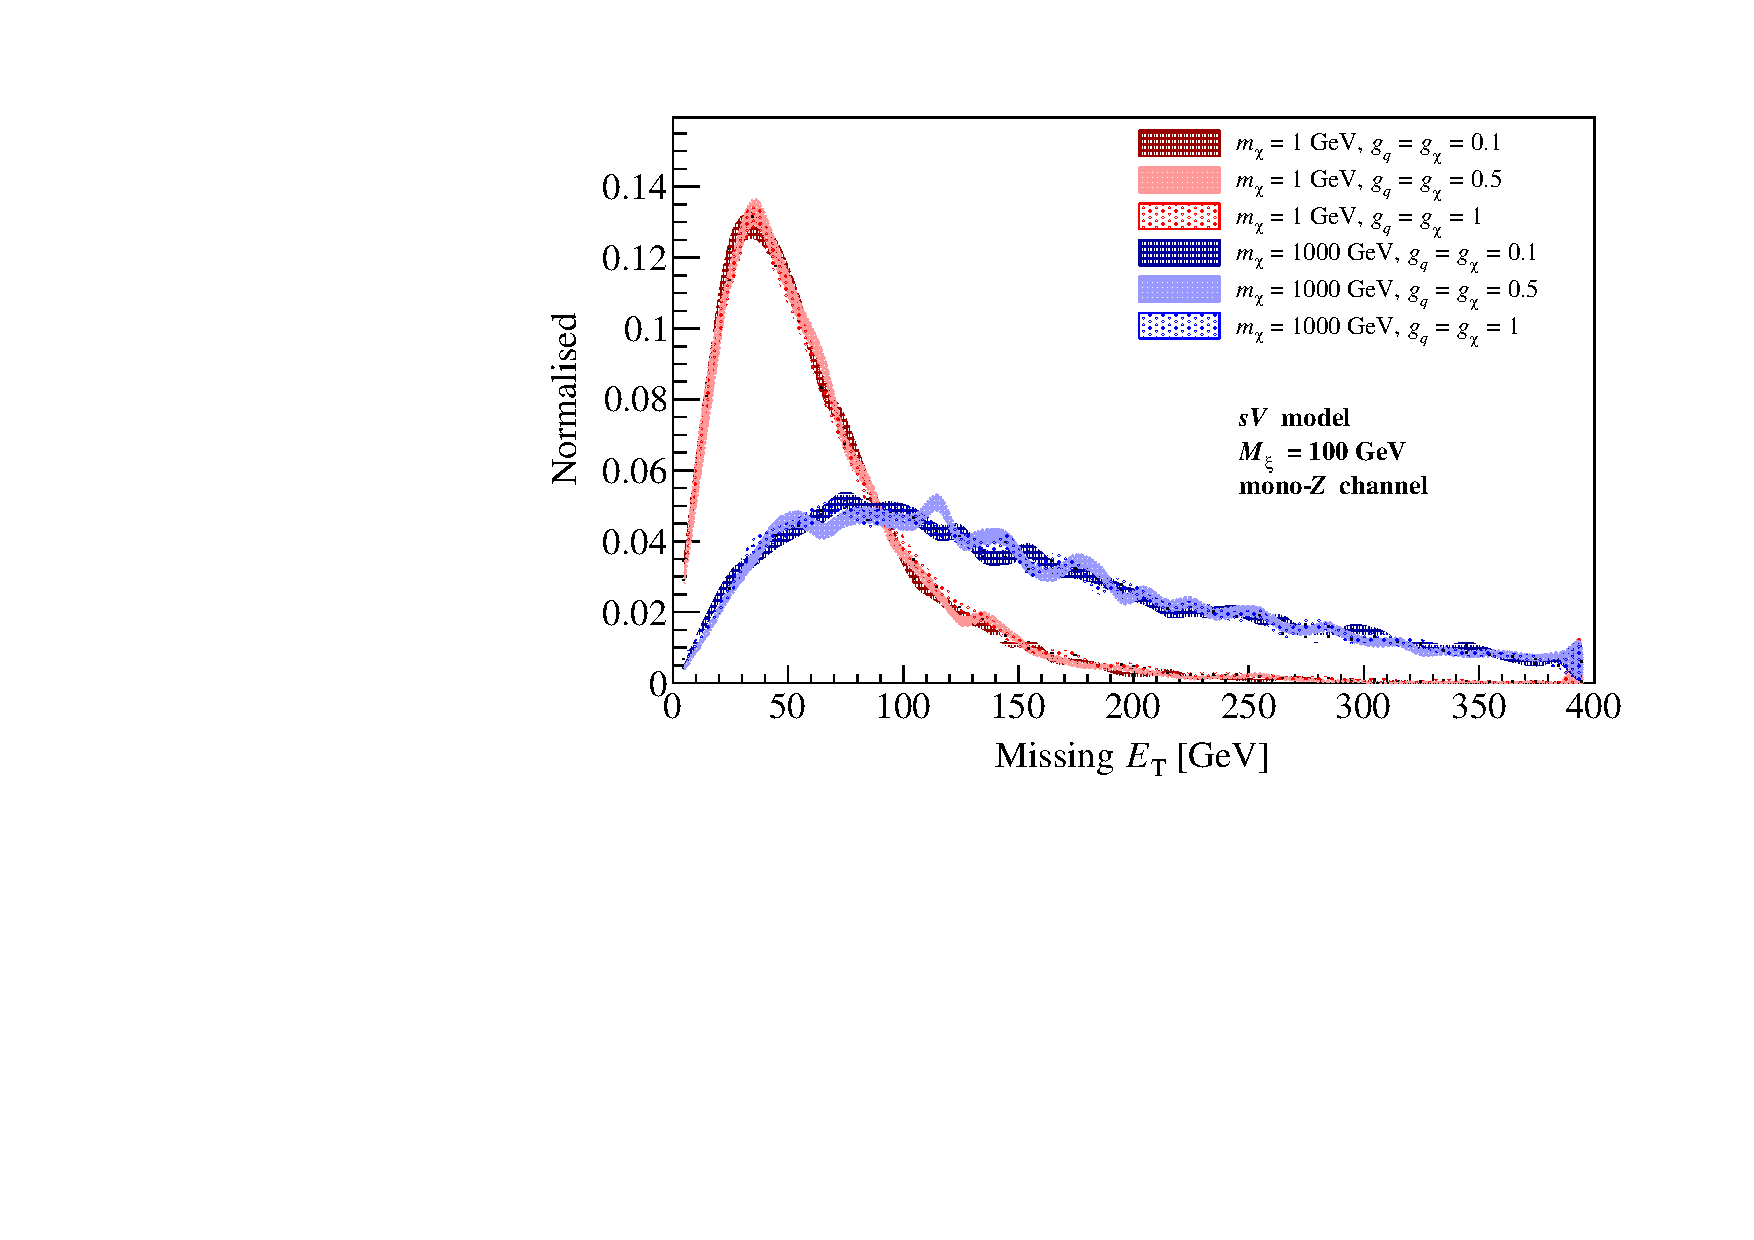
\includegraphics[width=0.45\textwidth]{figures/SVD_MET.pdf}
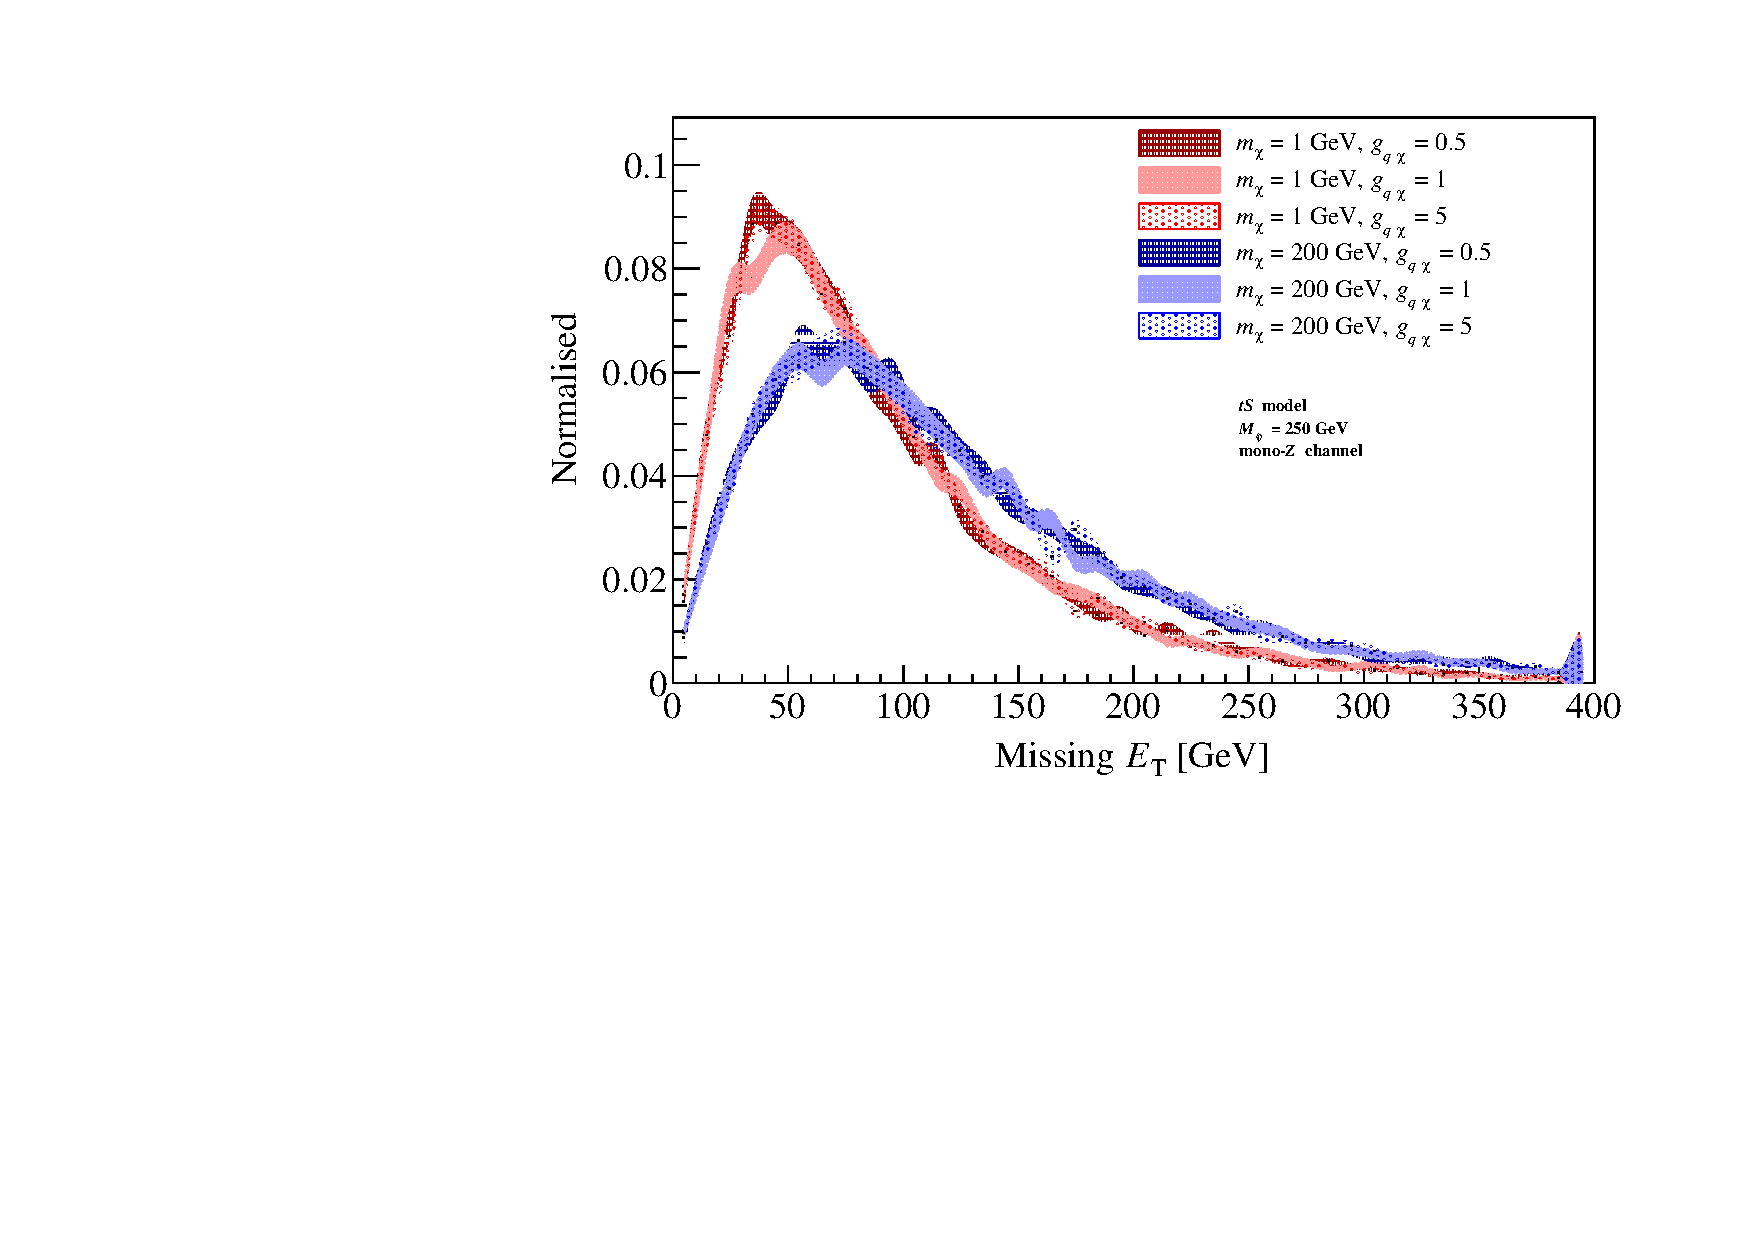
\includegraphics[width=0.45\textwidth]{figures/TSD_MET.pdf}
\caption{The $\met$ distribution showing the lack of dependence on the coupling (and hence the width) - possibly should include the widths on the plot.}
\label{MET_SVD_monoZ}
\end{center}
\end{figure}


%\textcolor{magenta}{This section should include:}
%\begin{enumerate}
%\item \textcolor{magenta}{Brief motivation for choice of simplified models? (eg. something like "we consider the most straightforward UV-completions of the D1, D5 and D8 effective operators, corresponding to the s-channel scalar, vector and axial-vector models respectively.}
%\item \textcolor{magenta}{The interaction Lagrangians for our four SiMs along with an explanation for why we only assume coupling to SM quarks.}
%\item \textcolor{magenta}{The assumptions and the decay widths associated with our models (?).}
%\item \textcolor{magenta}{Comments on the requirement that $\sqrt{g_{q}g_{\chi}} \leq 4\pi$ in order for the theory to remain perturbative? $\rightarrow$ comments on the choice of mass and coupling points used? Or does this belong in section \ref{sec:sec3}?}
%\end{enumerate}

%Resolving the mediator leads to two possibilities: the mediating particle is exchanged in the s-channel, in which case it may be colour neutral, or it is exchanged in the t-channel in which case it is necessarily coloured \cite{}. 

%\cite{ValidEFT, BeyondEFT, CSUSY} t-channel \cite{Buchmueller:2014yoa, SiM}.
